\documentclass{article}

\usepackage[utf8]{inputenc}
\usepackage[british]{babel}

\usepackage[adobe-utopia]{mathdesign}
\usepackage[series=z]{libgreek}
\usepackage{tgpagella}

\usepackage{amsmath}
\usepackage{tikz}
\usepackage{graphicx}
\usepackage{ntheorem}
\usepackage{enumitem}
\usepackage{stmaryrd}
\usepackage{xcolor}
\usepackage[colorlinks,citecolor=blue,linkcolor=blue,anchorcolor=blue,urlcolor=blue]{hyperref}
\usepackage{todonotes}
\usepackage{listings}
\lstset{
  xleftmargin=2pt,
  stepnumber=1,
  belowcaptionskip=\bigskipamount,
  captionpos=b,
  escapeinside={*'}{'*},
  language=haskell,
  tabsize=2,
  emphstyle={\bf},
  commentstyle=\it,
  stringstyle=\mdseries\rmfamily,
  showspaces=false,
  keywordstyle=\bfseries\rmfamily,
  columns=flexible,
  basicstyle=\small\sffamily,
  showstringspaces=false,
  morecomment=[l]\%,
}
\usetikzlibrary{arrows,calc,matrix,shapes}
\tikzset{every scope/.style={>=triangle 60,thick}}
\exhyphenpenalty 10000

\title{Connection Manager State Machine Specification}
\author{Marcin Szamotulski}

\tikzstyle{decision} =
  [ diamond
  , fill=green!255!blue!20
  , text width=4.5em
  , text badly centered
  , node distance=3cm
  , inner sep=0pt
  ]
\tikzstyle{outbound_state} =
  [ rectangle
  , rounded corners
  , fill=blue!60!white!70
  , minimum height=2em
  ]
\tikzstyle{inbound_outbound_state} =
  [ rectangle
  , rounded corners
  , fill=blue!60!red!50
  , minimum height=2em
  ]
\tikzstyle{inbound_state} =
  [ rectangle
  , rounded corners
  , fill=red!50
  , minimum height=2em
  ]
\tikzstyle{impossible_outbound_state} =
  [ rectangle
  , rounded corners
  , fill=blue!40!white!60
  , rounded corners
  , minimum height=2em
  ]
\tikzstyle{line} =
  [ draw
  , -latex'
  ]
\tikzstyle{error} =
  [ rectangle
  , rounded corners
  , fill=red!255!blue!20
  , minimum height=2em
  ]

\def\TCP{\textsf{TCP}}
\def\ipvfour{\textsf{ipv4}}
\def\ipvsix{\textsf{ipv6}}

% States
\def\InitialState{\textbullet}
\def\ReservedOutboundState{\texttt{ReservedOutboundState}}
\def\UnnegotiatedStateOut{\texttt{UnnegotiatedState Outbound}}
\def\UnnegotiatedStateIn{\texttt{UnnegotiatedState Inbound}}
\def\OutboundStateUni{\texttt{OutboundState Unidirectional}}
\def\OutboundStateDup{\texttt{OutboundState Duplex}}
\def\DuplexState{\texttt{DuplexState}}
\def\InboundStateUni{\texttt{InboundState Unidirectional}}
\def\InboundStateDup{\texttt{InboundState Duplex}}
\def\InboundStateAny{\texttt{InboundState dataFlow}}
\def\TerminatingState{\texttt{TerminatingState}}
\def\TerminatedState{\texttt{TerminatedState}}

% Transitions
\def\Reserve{\textsf{Reserve}}
\def\Connected{\textsf{Connected}}
\def\Accepted{\textsf{Accepted}}
\def\Overwritten{\textsf{Overwritten}}
\def\NegotiatedUniOut{$\text{\textsf{Negotiated}}^\text{\textsf{Unidirectional}}_\text{\textsf{Outbound}}$}
\def\NegotiatedDupOut{$\text{\textsf{Negotiated}}^\text{\textsf{Duplex}}_\text{\textsf{Outbound}}$}
\def\NegotiatedUniIn{$\text{\textsf{Negotiated}}^\text{\textsf{Unidirectional}}_\text{\textsf{Inbound}}$}
\def\NegotiatedDupIn{$\text{\textsf{Negotiated}}^\text{\textsf{Duplex}}_\text{\textsf{Inbound}}$}
% \def\NegotiatedDup{$\text{\textsf{Negotiated}}^\text{\textsf{Duplex}}$}
\def\PromotedToWarmDupLoc{$\text{\textsf{PromotedToWarm}}^\text{\textsf{Duplex}}_\text{\textsf{Local}}$}
\def\PromotedToWarmDupRem{$\text{\textsf{PromotedToWarm}}^\text{\textsf{Duplex}}_\text{\textsf{Remote}}$}
\def\DemotedToColdDupLoc{$\text{\textsf{DemotedToCold}}^\text{\textsf{Duplex}}_\text{\textsf{Local}}$}
\def\DemotedToColdDupRem{$\text{\textsf{DemotedToCold}}^\text{\textsf{Duplex}}_\text{\textsf{Remote}}$}
\def\DemotedToColdUniLoc{$\text{\textsf{DemotedToCold}}^\text{\textsf{Unidirectional}}_\text{\textsf{Local}}$}
\def\DemotedToColdUniRem{$\text{\textsf{DemotedToCold}}^\text{\textsf{Unidirectional}}_\text{\textsf{Remote}}$}
\def\Restart{\textsf{Restart}}
\def\Prune{\textsf{Prune}}
\def\PruneA{$\text{\textsf{Prune}}_\text{\textsf{1}}$}
\def\PruneB{$\text{\textsf{Prune}}_\text{\textsf{2}}$}
\def\PruneC{$\text{\textsf{Prune}}_\text{\textsf{3}}$}
\def\Terminate{\textsf{Terminate}}

% Peer states
\def\cold{\textit{cold}}
\def\warm{\textit{warm}}
\def\hot{\textit{hot}}
\def\established{\textit{established}}

% Component names
\def\ptopgov{\textit{p2p governor}}
\def\mux{\textit{mux}}
\def\inbgov{\textit{inbound protocol governor}}

% Utils

% TODO notes for the implementation
\newcommand{\todoimpl}[1]{\todo[backgroundcolor=red,linecolor=red]{#1}}

\begin{document}
\nocite{*}
\maketitle

\section{Introduction}
Connection manager is a component responsible for creating or accepting connections and keeping
track of their state.  Connection handler drives through handshake negotiation
and starts the multiplexer and will notify the connection manager about the
result of negotiation which triggers a state transitions.  From the point of
view of the connection manager it is only important whether a unidreictional
or duplex connection was negotiated.  Unidirectional connections, from
node-to-node protocol point of view, are ones which run either initiator or
responder side of mini-protocols exclusively, while duplex connections can run
either or both initiators and responders.  Note that in the outbound direction
(initiator side), it is \ptopgov{} which is responsible for deciding which set
of mini-protocols: \established{}, \warm{} or \hot{}, is running.  On the
inbound side (responder mini-protocols), we have no choice but to run all of
them.

The connection manager can be used in any \texttt{MuxMode}.
\texttt{InitiatorAndResponder} mode is useful for managing connection with
external nodes (\textit{node-to-node protocol}), while \texttt{ResponderMode}
is useful for running a server which responds to local connections
(\textit{node-to-client protocol}).

Connection manager can use at most one \ipvfour{} and at most one \ipvsix{}
address.  It will bind to the correct address depending on the remote address
type (\ipvfour{}/\ipvsix{}).

In this specification we will often need to speak about two nodes communicating
via a \TCP{} connection.  We will often call them local and remote ends of the
connection or local \slash{} remote nodes; we will usually take the
perspective of the local node.

\section{Components} 
\begin{figure}[h]
  \footnotesize
  \def\xa{-2.5}
  \def\xb{2.5}
  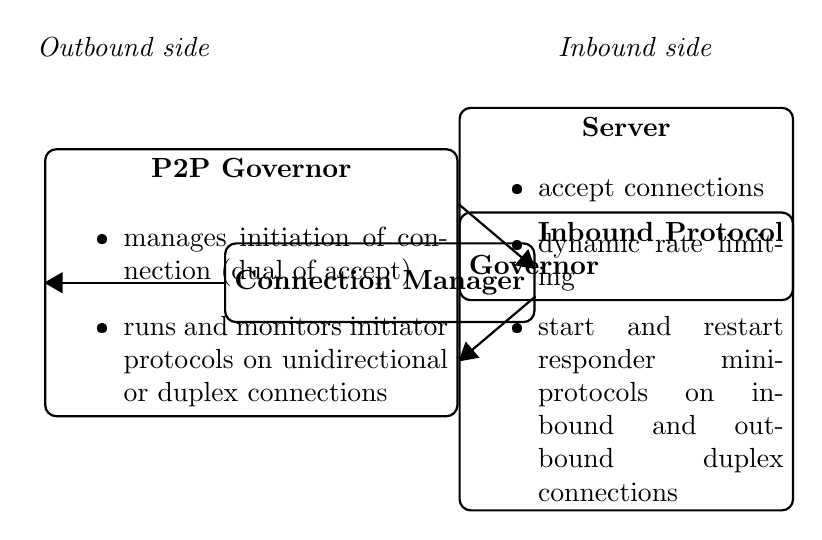
\begin{tikzpicture}
    \node at (-3.25, 0)  {\textit{Outbound side}};
    \node at ( 3.25, 0)  {\textit{Inbound side}};

    \node[rounded corners, rectangle, draw, minimum height=3cm,anchor=east] (p2p_governor) at (\xa, -3)
     {\begin{minipage}{5cm}
       \hfill\textbf{P2P Governor}\hfill
       \vspace{0.5em}
      \begin{itemize}
        \item manages initiation of connection (dual of accept)
        \item runs and monitors initiator protocols on unidirectional or duplex connections
      \end{itemize}
      \end{minipage}};

    \node[rounded corners, rectangle, draw, anchor=west] (server) at (\xb, -2)
      {\begin{minipage}{4cm}
        \hfill{\textbf{Server}}\hfill
        \vspace{0.2em}
        \begin{itemize}
          \item accept connections
          \item dynamic rate limiting
        \end{itemize}
      \end{minipage}};

    \node[rounded corners, rectangle, draw, anchor=west] (inbound_governor) at (\xb, -4)
      {\begin{minipage}{4cm}
        \hfill{\textbf{Inbound Protocol Governor}}\hfill
        \vspace{0.2em}
          \begin{itemize}
            \item start and restart responder mini-protocols on inbound and
              outbound duplex connections
          \end{itemize}
      \end{minipage}};

    \node[rounded corners, rectangle, draw, minimum height=1cm] (connection_manager) at (0, -3) {\textbf{Connection Manager}};

    \draw[<-] (p2p_governor)           -- (connection_manager);
    \draw[->] (server.west)            -- (connection_manager.5);
    \draw[->] (connection_manager.355) -- (inbound_governor.west);
  \end{tikzpicture}
\end{figure}

\section{Connection Manager}

Connection manager exposes two methods two register a connection:
\begin{lstlisting}
type IncludeOutboundConnection peerAddr handle handleError m
    = peerAddr -> m (Connected peerAddr handle handleError)

type IncludeInboundConnection  socket peerAddr handle handleError m
    = socket -> peerAddr -> m (Connected peerAddr handle handleError)
\end{lstlisting}
The first one asks the connection manager to either connect a peer or if
possible reuse a duplex connection.  The other one allows to register an
inbound connection, which was \texttt{accepted}.  Both methods are blocking
operations and return either an error (handshake negotiation error or
a multiplexer error) or a handle to a \textit{negotiated} connection.


\section{Connection states}

Each connection is either initiated by \texttt{Inbound} or \texttt{Outbound} side.
\begin{lstlisting}
data Provenance
  = Inbound
  | Outbound
\end{lstlisting}
Each connection negotiates \texttt{dataFlow}:
\begin{lstlisting}
data DataFlow
  = Unidirectional
  | Duplex
\end{lstlisting}
Negotiation of \texttt{DataFlow} is done by the handshake protocol, the final
result depends on two factors: negotiated version and \texttt{InitiatorOnly}
flag which is announced through handshake.  Each connection can be in one
of the following states:
\begin{lstlisting}
data ConnectionState
  -- Connection manger is about to connect to a peer.
  = ReservedOutboundState

  -- Connected to a peer, handshake negotiation is ongoing.
  | UnnegotiatedState Provenance

  -- Inbound connection has been negotiated.
  | InboundState DataFlow

  -- Outbound connection has been negotiated.
  | OutboundState DataFlow

  -- Connection runs in duplex mode: either outbound connection negotiated
  -- 'Duplex' data flow, or 'InboundState Duplex' was reused.
  | DuplexState

  -- Connection has terminated; socket is released, thread running the
  -- connection is closed.  For some small delay the connection is kept in this
  -- state until the kernel releases all the resources.
  | TerminatingState

  -- Connection is removed from connection manager map, at this point the
  -- connection manager can create a new connection to that peer.
  | TerminatedState
\end{lstlisting}
The above type is a stripped version of what is implemented.  The real
implementation tracks more detail, e.g. connection id (the quadruple of ip
addresses and ports), muliplexer handle, etc.

\begin{figure}[p]\label{fig:statediagram}
  {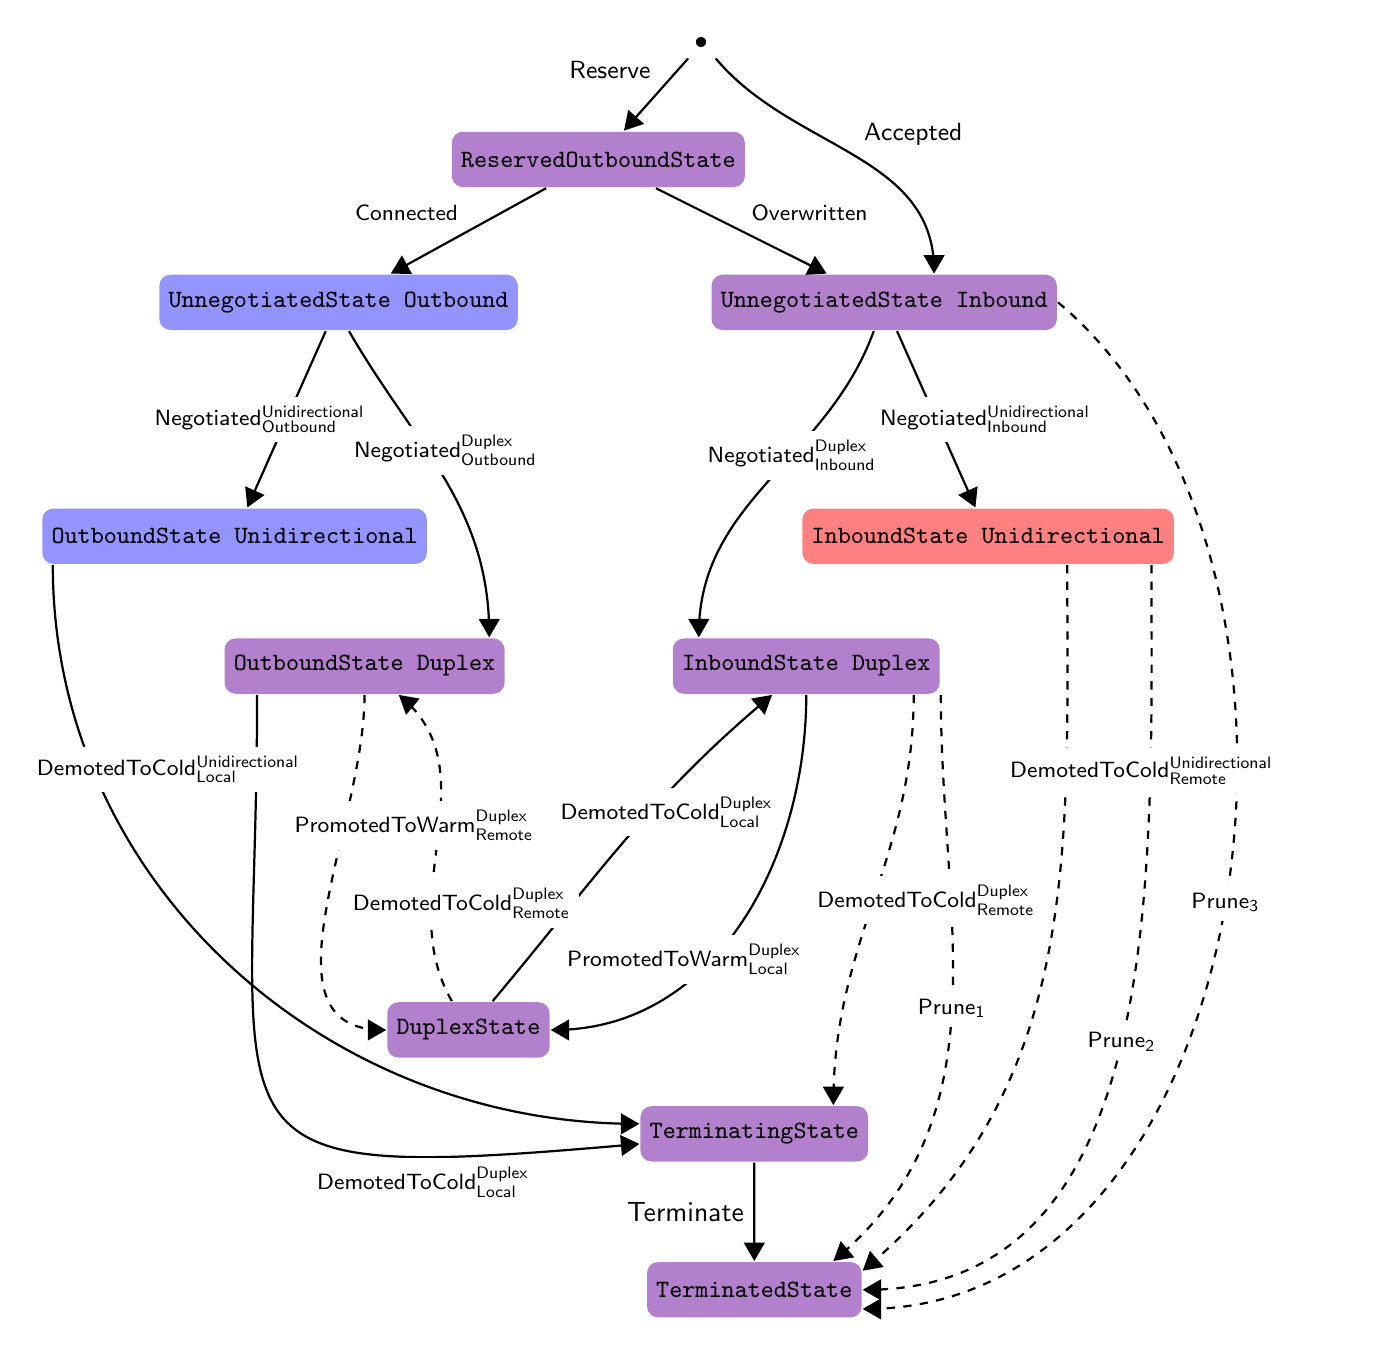
\begin{tikzpicture}[scale=0.66]
    \node                         (init)                       at ( 2,   2)    {\small\InitialState};
    \node[inbound_outbound_state] (ReservedOutboundState)      at ( 0,-0.25)   {\small\ReservedOutboundState};
    \node[outbound_state]         (UnnegotiatedState_Outbound) at (-5,  -3)    {\small\UnnegotiatedStateOut};
    \node[inbound_outbound_state] (UnnegotiatedState_Inbound)  at ( 5.5, -3)   {\small\UnnegotiatedStateIn};
    \node[outbound_state]         (OutboundState_UniDF)        at (-7, -7.5)   {\small\OutboundStateUni};
    \node[inbound_outbound_state] (OutboundState_DupDF)        at (-4.5,  -10) {\small\OutboundStateDup};
    \node[inbound_state]          (InboundState_UniDF)         at ( 7.5, -7.5) {\small\InboundStateUni};
    \node[inbound_outbound_state] (InboundState_DupDF)         at ( 4,  -10)   {\small\InboundStateDup};
    \node[inbound_outbound_state] (DuplexState)                at (-2.5, -17)  {\small\DuplexState};
    \node[inbound_outbound_state] (TerminatingState)           at ( 3,  -19)   {\small\TerminatingState};
    \node[inbound_outbound_state] (TerminatedState)            at ( 3,  -22)   {\small\TerminatedState};


    \draw[->] (init) -- node[fill=white,pos=0.425,above left]{\small\Reserve} (ReservedOutboundState);
    \draw[->] (init) to [out=310, in=90] node[fill=white, above right]{\small\Accepted}                      (UnnegotiatedState_Inbound.30);

    \draw[->] (ReservedOutboundState)          -- node[fill=white,above left] {\footnotesize\Connected}             (UnnegotiatedState_Outbound);
    \draw[->] (ReservedOutboundState)          -- node[fill=white,above right] {\footnotesize\Overwritten}          (UnnegotiatedState_Inbound);

    \draw[->] (UnnegotiatedState_Outbound)     -- node[fill=white,left=-32pt] {\footnotesize\NegotiatedUniOut}      (OutboundState_UniDF);
    \draw[->] (UnnegotiatedState_Outbound.290) to [out=-60, in=90]
                                                  node[fill=white,right=-30pt,pos=0.4]{\footnotesize\NegotiatedDupOut} (OutboundState_DupDF.13);

    \draw[->] (UnnegotiatedState_Inbound)      -- node[fill=white,right=-24pt]{\footnotesize\NegotiatedUniIn}       (InboundState_UniDF);
    \draw[->] (UnnegotiatedState_Inbound)      to [out=-110, in=90]
                                                  node[fill=white,pos=0.4]{\footnotesize\NegotiatedDupIn} (InboundState_DupDF.165);

    \draw[->, dashed] (UnnegotiatedState_Inbound.360)
                                               to [out=320, in=0]   node[fill=white]{\footnotesize\PruneC}                                   (TerminatedState.350);
    \draw[->, dashed] (InboundState_DupDF.348) to [out=270, in=40]  node[fill=white]{\footnotesize\PruneA}                                   (TerminatedState.20);
    \draw[->, dashed] (InboundState_UniDF.350) to [out=270, in=0]   node[fill=white]{\footnotesize\PruneB}                                   (TerminatedState.0);
    \draw[->, dashed] (InboundState_UniDF.340) to [out=270, in=40]  node[fill=white,pos=0.25,right=-24pt]{\footnotesize\DemotedToColdUniRem} (TerminatedState.10);
    \draw[->, dashed] (InboundState_DupDF.345) to [out=270, in=90]  node[fill=white,pos=0.5,right=-24pt]{\footnotesize\DemotedToColdDupRem}  (TerminatingState.20);

    \draw[->]         (OutboundState_DupDF.195) to [out=-90,in=-175,looseness=2] node[fill=white,pos=0.8,below]{\footnotesize\DemotedToColdDupLoc}
                                                                                                                                                (TerminatingState.185);
    \draw[->]         (DuplexState)            to [out=50,in=220]  node[fill=white,pos=0.6,left=-48pt]{\footnotesize\DemotedToColdDupLoc}       (InboundState_DupDF);
    \draw[->]         (InboundState_DupDF)     to [out=-90,in=0]   node[fill=white,pos=0.6,right=-56pt]{\footnotesize\PromotedToWarmDupLoc}     (DuplexState);
    \draw[->, dashed] (DuplexState)            to [out=120,in=-40] node[fill=white,right=-32pt,pos=0.3]{\footnotesize\DemotedToColdDupRem}      (OutboundState_DupDF);
    \draw[->, dashed] (OutboundState_DupDF)    to [out=-90,in=180] node[left,fill=white,pos=0.3,left=-72pt]{\footnotesize\PromotedToWarmDupRem} (DuplexState);

    \draw[->] (OutboundState_UniDF.189)        to [out=270, in=180,pos=0.23] node[fill=white,right=-24pt]{\footnotesize\DemotedToColdUniLoc}    (TerminatingState.175);

    \draw[->] (TerminatingState) -- node[fill=white,left]{\Terminate} (TerminatedState);
  \end{tikzpicture}}
  \caption{\textit{Inbound} (blue \& violet) and \textit{outbound} (red \&
  violet) connection states and allowed transitions.  Dashed arrows indicate an
  asynchronous transition, either driven by the decision of a remote peer
  (\DemotedToColdUniRem{} and \DemotedToColdDupRem{}) or the local connection
  manager itself (\PruneA{}, \PruneB{} and \PruneC{}).}
\end{figure}

Figure~\ref{fig:statediagram} shows all the transitions between
\texttt{ConnectionState}s.  Blue and violet states represent states of
an \textit{outbound} connection, red and violet represent states of an
\textit{inbound} connection.  Dashed arrows indicated an asynchronous
transitions which are triggered either by remote node or by the connection
manger itself.

Note that the vertical symmetry in the graph corresponds to local / remote
state of the connection:

\begin{table}[h]
  \begin{tabular}[h]{l|l}
    \textit{local connection state} &  \textit{remote connection state}    \\ [0.3em]
    \hline \\ 
    \UnnegotiatedStateOut{}         &  \UnnegotiatedStateIn{}              \\ [0.2em]
    \OutboundStateUni{}             &  \InboundStateUni{}                  \\ [0.2em]
    \OutboundStateDup{}              &  \InboundStateDup{}                 \\ [0.2em]
    \DuplexState{}                  &  \DuplexState{}                      \\ [0.2em]
  \end{tabular}
\end{table}


\section{Transitions}

\subsection{\Reserve{}}
When connection manager is asked for an outbound connection, it reserves a slot
in its state for that connection.  If any other thread will ask for the same
outbound connection, the connection manager will raise an exception in that thread.
Reservation is done to guarantee exclusiveness for state transitions to
a single outbound thread.

\subsection{\Connected{}}
This transition is executed once an outbound connection successfully performed
\texttt{connect} system call. 

\subsection{\Accepted{} and \Overwritten{}}
Transition driven by \texttt{accept} system call.  Once it returns the
connection manager might either not know about such connection or be in
\ReservedOutboundState{}.  \Accepted{} transition represents the former
situation while the latter is captured by \Overwritten{} transition.

Let us note that if \Overwritten{} transition happened, then on the outbound
side the scheduled \texttt{connect} call will fail.  In this case the
\ptopgov{} will recover, put the peer in a queue of failed peers, and
will either try to connect to another peer or reconnect to that peer after some
small delay in which case it would re-use the accepted connection (assuming that
duplex connection was negotiated).

\subsection{\NegotiatedUniOut{} and \NegotiatedDupOut{}}
Once an outbound connection has been negotiated one of \NegotiatedUniOut{} or
\NegotiatedDupOut{} is performed, depending on the result of handshake
negotiation.  Duplex connections are negotiated only for node-to-node protocol
version higher than \texttt{NodeToNodeV\_4}\todoimpl{the exact version number will change} and neither
side declared that it is an initiator only.

If duplex outbound connection was negotiated, the \textit{connection manager}
needs to ask the \textit{inbound protocol governor} to start and monitor
responder mini-protocols on the outbound connection.

\subsection{\NegotiatedUniIn{} and \NegotiatedDupIn{}}
This transition is performed once handshake negotiated a unidirectional or
duplex connection on an inbound connection.  The \textit{inbound protocol
governor} will start all responder protocols (for all \established{}, \warm{}
and \hot{} groups of mini-protocols) and keep monitoring them.

\subsubsection{Unidirectional connection}
If a unidirectional connection was negotiated and both \ptopgov{} and
\textit{inbound protocol governor} were awaiting for the negotiation we should
let the governor to take advantage of the connection.   Outbound connections
which are result of the \ptopgov{} are more valuable to the running
system.

\todo[inline,backgroundcolor=red,linecolor=red]{
The current implementation does not follow this requirement.  An implementation
of it would require to detect the race condition in a relabile way using
\texttt{stm} transactions.}

\subsection{\DemotedToColdUniLoc{}}
This transition is driven by the \ptopgov{}: when it decides to demote the peer
to \cold{} state.  This transition should trigger a normal \TCP{} termination,
via \texttt{close} call: we started the connection, and thus we are in position
to close it.

\subsection{\DemotedToColdDupLoc{}}
As above this transition is driven by the local \ptopgov{}, but this time it is
triggered on a connection in \texttt{DuplexState}.  The \textit{connection
manager} will need to be instructed to change the connection state.

\subsection{\PromotedToWarmDupLoc{}}
This transition is driven by the local \ptopgov{} when it promotes a \cold{} peer
to \warm{} state.  This is the case where a connection manager will provide
a handle to an existing connection to the \ptopgov{}.

\subsection{\DemotedToColdUniRem{}, \DemotedToColdDupRem{}}
The \DemotedToColdUniRem{} and the two \DemotedToColdDupRem{} transitions are triggered
when the remote end demotes the local peer to \cold{}.  The \inbgov{} can
notice this when one of the \established{} protocols returns.  It will need to
update the connection manager that this transition happend.  For the
\DemotedToColdDupRem{} from \InboundStateDup{} there is a potential race
condition which side will call \texttt{close} first.  For this reason it is
safer to transition to \TerminatingState{}.  For \DemotedToColdDupRem{} from
\InboundStateUni{} we expect that the remote side will call \texttt{close} as
soon as it terminated all its \established{} mini-protocols, thus we can
directly transition to \TerminatedState{} since our socket should not be held
in \texttt{TIME\_WAIT} state.
\todoimpl{Implementation review is required.}

\subsubsection{Restarting a mini-protocol}
When the server restarts a responder side of a mini-protocol is not a visible
state transition to the governor but it deserves to be described.  The actions
depend on the state in which is the connection:

\paragraph{\DuplexState{}:}
if any responder side of a mini-protocol returns, we
restart it.  This must be a result of either \warm{} to \hot{}, \hot{} to
\warm{} or a transition to \cold{}.  In \DuplexState{} we don't need to
distinguish them: in either case the local \ptopgov{} is still using this
connection.  Note that even in the case of being demoted to \cold{} (and thus
executing \DemotedToColdDupRem{} transition), we restart all the
mini-protocols.

\paragraph{\InboundStateAny{}:}
in these states we need to distinguish remote transtions between \warm{} and
\hot{} and transtions to \cold{}.  In the latter case a mini-protocol shall be
restarted, in the former the \inbgov{} needs to trigger termination procedure:
await with a timeout for all mini-protocols to terminate, when that happens
check once again whether connection is not in \DuplexState{} and trigger one of
\DemotedToColdDupRem{} or \DemotedToColdUniRem{} transition.

We can distinguish transition remote transitions to \cold{} state from
transitions between \warm{} and \hot{} states simply by noticing that an
\established{} mini-protocol terminated.

\subsection{\PromotedToWarmDupRem{}}
This transition is triggered by the remote peer, and thus is asynchronous.  The
\inbgov{} can notice it by observing multiplexer ingress side of \established{}
mini-protocols.  It then should notfiy the \textit{connection manager}.

\subsection{\Prune{} transitions}
\todoimpl{Not implemented}
First let us note that a connection in \InboundStateDup{}, the initial
state of \PruneA{} transition, could have been initiated by either side.  This
means that even though a node might have not accepted any connection it could
end up serving peers and go beyond server hard limit and thus exceed the number
of file descriptors.  This is thanks to the path: \Connected{},
\NegotiatedDupOut{}, \PromotedToWarmDupRem{} \DemotedToColdDupLoc{}, which
leads from the initial outbound state to \InboundStateDup{}, the same state in
which accepted duplex connections end up.  Even though the server rate limits
connections based on how many connections are in this state, we could end up
exceeding server hard limit.

To solve this problem, when a connection is transitioned from 
\DuplexState{} to \InboundStateDup{} (via \DemotedToColdDupLoc{}) the
connection manager will check if we the server hard limit was exceeded.  If
that happened, the connection manager will reset one connection in either
\InboundStateDup{}, \InboundStateUni{} or \UnnegotiatedStateIn{}.  This
corresponds to one of the \PruneA{}, \PruneB{} or \PruneC{} transitions.  If we
keep the number of \established{} peers to be smaller than the server hard
limit, we should never need to reset a connection in \DuplexState{}.

We prefer to reset inbound connections rather than close an outbound connection
because from systemic point of view, outbound connections are more valuable
than inbound ones.

The \textit{inbound protocol governor} is able to make an educated decision
which connection to reset, hence it should help make the right decision.
Initially, we aim for a decision driven by randomness, but other choices are
possible; we can take into account whether we are \hot{} to the remote end, or
for how long we have been \hot{} to them.

\subsection{\TerminatingState{} and \TerminatedState{}}
\todoimpl{The terminating state is not implemented.}
After a connection was closed we keep it in \TerminatingState{} for some time.
This allows for the kernel to release all the resources (addresses).  After
this fixed timeout the connection is removed from the connection manager
state, which we explicitely signify in this specification as
\TerminatedState{}.

\todo[inline]{
How to avoid problem of keeping a connection in \TerminatingState{} for too
long or keeping connection in \texttt{TIME\_WAIT} state? 

This would be problematic when restarting a node (without rebooting the
system) with adjusted configuration.  Even in clean shutdown of all protocols,
the node that initialised the shutdown will endup in \texttt{TIME\_WAIT} state.
Useing ephemeral ports for local peers solves this.
}

\subsection{Protocol errors}
If a mini-protocol errors, on either side, connection will be reset (as oposed
to \texttt{close}), and put in \TerminatedState{}.  This can possibly happen in
any connection state.

{\small
Note for implementation: reseting conndtion should be the default.  It can be
set with \texttt{SO\_LINGER} option with a zero linger interval.  This will
cause \texttt{close} call to include \texttt{RST} \TCP{} header.  There are
only two cases where we need \texttt{close} rater than \texttt{reset}:
\DemotedToColdUniLoc{} and \DemotedToColdDupLoc{}.
\todoimpl{Needs to be implemented.}
}

\section{\textit{Outbound} connection}

The state of a connection when \texttt{includeoutboundConnection} is called
which leads to either \OutboundStateUni{} or \DuplexState{} must be either:
\ReservedOutboundState{}, \UnnegotiatedStateIn{} or
\InboundStateDup{}.
\paragraph{\textnormal{initial state (\InitialState{})}:} the connection manager does not have
  a connection with that peer.  The  connection is put \ReservedOutboundState{}
  before connection manager connects to that peer;

\paragraph{\UnnegotiatedStateIn{}:} if the connection manager accepted
  a connection from that peer, handshake is ongoing;

\paragraph{\InboundStateDup{}:} if connection manager accepted connection from
  that peer and handshake negotiated a \texttt{Duplex} data flow;

\paragraph{\TerminatingState{}:} \todo[inline]{Not yet specified: either wait for for
\TerminatedState{} or throw an exception.}

\paragraph{\textnormal{Otherwise}:} if connection manager is asked to connect ot
peer and there exists a connection which is in any other state connection
manager signals the caller with an error.

\paragraph{}
Figure~\ref{fig:outbound_flow} shows inbound connection state evolution.  This
shows the exact steps and decisions that \texttt{includeOutboundConnection}
needs to make.

\begin{figure}[p]\label{fig:outbound_flow}
  \footnotesize{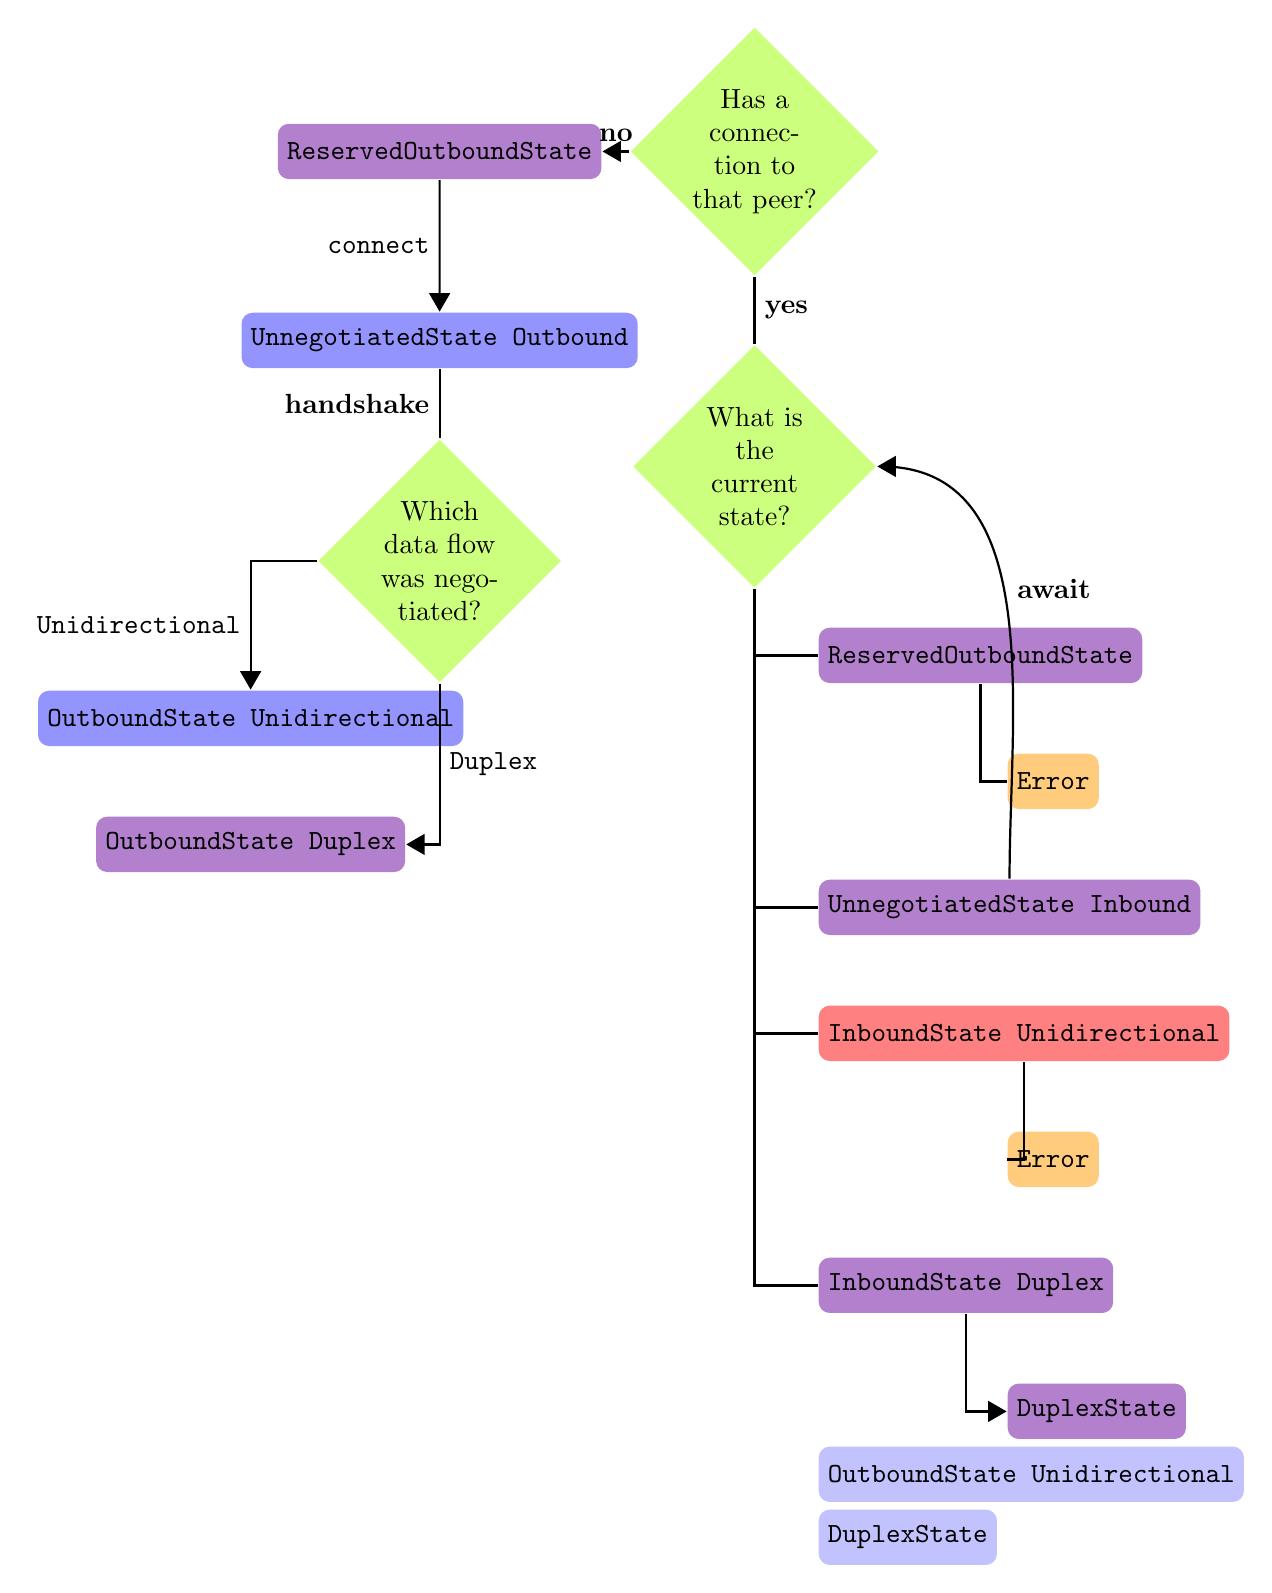
\begin{tikzpicture}[scale=0.8]
    \node[decision]               (init)      at (0,0) {Has a connection to that peer?};
    \node[inbound_outbound_state] (not_found) at (-5, 0) {\ReservedOutboundState{}};

    % Connection not found flow
    \draw[->] (init) -- node[above] {\textbf{no}}  (not_found);
    \node[outbound_state] (connected) at (-5, -3) {\UnnegotiatedStateOut{}};
    \draw[->] (not_found) -- node[left] {\textbf{\texttt{connect}}} (connected);

    % This may be influenced by `initiator only` flag or version of the connection.
    \node[decision]               (handshake_decision_outbound) at (-5, -6.5) {Which data flow was negotiated?};
    \node[outbound_state]         (outbound_unidf)              at (-8, -9)   {\OutboundStateUni{}};
    \draw (connected) -- node[left] {\textbf{\textbf{handshake}}} (handshake_decision_outbound);

    \node[inbound_outbound_state] (outbound_dupdf)             at (-8, -11)  {\OutboundStateDup{}};
    \draw[->] (handshake_decision_outbound.west) -| node[left, near end] {\texttt{Unidirectional}} (outbound_unidf);
    \draw[->] (handshake_decision_outbound) |- node[right, near start] {\textbf{\texttt{Duplex}}} (outbound_dupdf);

    % Connection found flow

    \node[decision] (found) at (0, -5)     {What is the current state?};
    \draw (init) -- node[right] {\textbf{yes}} (found);

    \node[inbound_outbound_state,anchor=west] (reserved_outbound) at (1, -8)  {\ReservedOutboundState};
    \node[error,anchor=west]                  (termination_c)     at (4, -10) {\textbf{\texttt{Error}}};
    \draw   (found.south)       |- (reserved_outbound);
    \draw[] (reserved_outbound) |- (termination_c);

    \node[inbound_outbound_state,anchor=west] (unnegotiated_inbound) at (1, -12) {\UnnegotiatedStateIn};
    \draw (found.south) |- (unnegotiated_inbound.west);
    \draw[->] (unnegotiated_inbound) to[out=90,in=0] node[above right] {\textbf{await}} (found.east);

    \node[inbound_state,anchor=west] (inbound_unidf) at (1, -14) {\InboundStateUni};
    \node[error,anchor=west] (termination_unidf) at (4, -16) {\textbf{\texttt{Error}}};
    \draw (found.south) |- (inbound_unidf);
    \draw[] (inbound_unidf) |- (termination_unidf);

    \node[inbound_outbound_state,anchor=west] (inbound_dupdf) at (1, -18) {\InboundStateDup};
    \node[inbound_outbound_state,anchor=west] (duplex)        at (4, -20) {\DuplexState};
    \draw (found.south) |- (inbound_dupdf);
    \draw[->] (inbound_dupdf) |- (duplex);


    \node[impossible_outbound_state,anchor=west] (outbound_imp) at (1, -21) {\OutboundStateUni};
    \node[impossible_outbound_state,anchor=west] (duplex_imp)   at (1, -22) {\DuplexState};

  \end{tikzpicture}}
  \caption{\textit{Outbound} connection flow graph}
\end{figure}

\subsection{\OutboundStateDup{} and \DuplexState{}}
Once an outbound connection negotiates \texttt{Duplex} data flow it is directly
put in \OutboundStateDup{}.
At this point we need to start responder protocols.  This means that the
connection manager needs a way to inform server (which accepts and monitors
inbound connections), to start the protocols and monitor that connection.  It
is transitioned to \DuplexState{} once we notice any incoming traffic on any
of \established{} protocols.

The implementation is using
\href{https://github.com/input-output-hk/ouroboros-network/blob/coot/connection-manager/ouroboros-network-framework/src/Ouroboros/Network/ConnectionManager/Server/ControlChannel.hs\#L123}{\texttt{TBQueue}}.
Server is using this channel for monitoring inbound connections which includes
starting responder protocols.

\subsection{Termination}\label{sec:outbound_termination}

When \ptopgov{} demotes a peer to \cold{} state an outbound
connection needs to transition either from \OutboundStateUni{} to
\TerminatingState{} or from \DuplexState{} to \InboundStateDup{}.  To
support that the connection manager exposes a method:
\begin{lstlisting}
unregisterOutboundConnection :: peerAddr -> m ()
\end{lstlisting}
This method checks the connection state and either shuts down the multiplexer
and closes the \TCP{} connection, or just changes the state of the connection.


\section{\textit{Inbound} connection}

Initial states for inbound connection is either:

\begin{itemize}
  \item \UnnegotiatedStateIn{}
  \item \ReservedOutboundState{}

    This can happen when \texttt{includeOutboudConnection} reserves
    a connection with \ReservedOutboundState{}, but before it calls
    \texttt{connect} the \texttt{accept} call would return.  In this case, the
    \texttt{connect} call will fail and, as a consequence,
    \texttt{includeOutboundConnection} will fail too.  Any mutable variables
    used by it can be disposed, since there is no thread that could be blocked
    on it: if there was another thread that called
    \texttt{includeOutboundConnection} it would see \ReservedOutboundState{}
    and it would throw.

    To make sure that this case is uncommon, we need to guarantee that the
    connection manager does not block between putting the connection in the
    \ReservedOutboundState{} and calling the \texttt{connect} system call.
\end{itemize}

\begin{figure}[h]
  \footnotesize{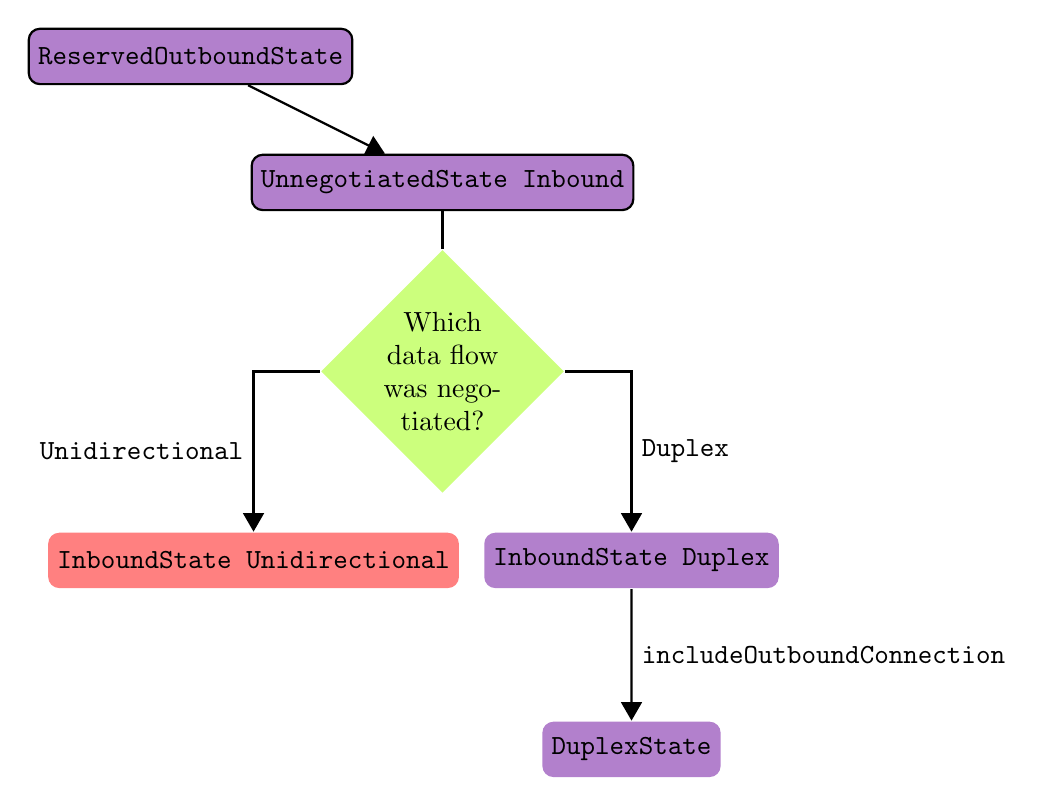
\begin{tikzpicture}[scale=0.8]
    \node[inbound_outbound_state,draw] (reserved_outbound)    at (-4, 0) {\ReservedOutboundState};
    \node[inbound_outbound_state,draw] (unnegotiated_inbound) at (0, -2)  {\UnnegotiatedStateIn};
    \draw[->] (reserved_outbound) -- (unnegotiated_inbound);

    \node[decision] (handshake_decision_inbound) at (0, -5) {Which data flow was negotiated?};
    \draw (unnegotiated_inbound) -- (handshake_decision_inbound);
    \node[inbound_state]          (inbound_unidf) at (-3, -8) {\InboundStateUni{}};
    \node[inbound_outbound_state] (inbound_dupdf) at (3,  -8) {\InboundStateDup{}};
    \draw[->] (handshake_decision_inbound.west) -| node[left, near end]{\textbf{\texttt{Unidirectional}}} (inbound_unidf);
    \draw[->] (handshake_decision_inbound.east) -| node[right,near end]{\textbf{\texttt{Duplex}}}         (inbound_dupdf);

    \node[inbound_outbound_state] (duplex) at (3, -11) {\DuplexState{}};
    \draw[->] (inbound_dupdf) -- node[right]{\textbf{\texttt{includeOutboundConnection}}} (duplex);
  \end{tikzpicture}}
  \caption{\textit{Inbound} connection flow graph, both bordered states:
  \ReservedOutboundState{} and \texttt{UnnegotiatedState prov} can be the
  initial states.}
\end{figure}

\section{Server}

Server is the primary component which will use
\texttt{includeInboundConnection}.  When \texttt{includeInboundConnection}
successfully returns the server has access to mux handle which allows to start
responders of all mini-protocols.  The server needs not only to start them but
also monitor them.  The remote peer might promote / demote the node which will
terminate some of the protocols and require others to be responsive.  This
means that the server needs also to monitor all mini-protocols and restart them
when need.

\subsection{Termination}

\subsubsection{Clean termination}
Termination of a connection can be done from
the two states: \InboundStateAny{}.  The
connection manager shall be instructed to terminate the connection only when
any \established{} mini-protocols terminated.  When the connection was in
\InboundStateDup{} and all responder mini-protocol reached their terminal
states, it might happen that the \ptopgov{} started promoting the peer to
\warm{} state, in which case, the \inbgov{} is responsible for making all
responder sides up.

Termination procedure starts when the \inbgov{} detects termination of one of
the \established{} protocols.   It then awaits for all other protocols to
terminate, or the connection manger changes the state of the connection to
\DuplexState{}, or the operation timeouts.  If all protocols terminated the
connection is closed and transitioned to
\TerminatingState{}.  If timeout was reach the connection is reset and ptu int
\TerminatedState{}.  If the connection was promoted to \DuplexState{} all
protocols which terminated are restarted.

For this reason the connection manager needs to expose the following methods
\begin{lstlisting}
data IsInDuplexState m
  = InDuplexState
  | AwaitForDuplexState (STM m ())

isNotDuplexState :: peerAddr -> STM m (IsInDuplexState m)

-- | Terminates the connection, returns 'True' if succeeds, 'False' if the
-- connection is in 'Duplex' state.
unregisterInboundConnection :: peerAddr -> m Bool
\end{lstlisting}

The 'isNotDuplexState' operation is a non blocking operation which returns
\texttt{InDuplexState} iff the \texttt{peerAddr} connection is in \DuplexState{}.
If the connection is in \texttt{InboundState dataFlow} it returns an
\texttt{STM} action which blocks until the connection changes its state to
\DuplexState{}.  In particular if the initial state was
\InboundStateUni{} it returns \texttt{retry :: STM m ()}.
This allows us to construct and stm action which is first to finish
synchronisation between three events:
\begin{itemize}
  \item all responder mini-protocols terminate
  \item timeout fires
  \item connection is promoted to \DuplexState{}
\end{itemize}

\subsubsection{Forceful termination}
The connection manager might reset an inbound connection through one of the
\PruneA{}, \PruneB{}, \PruneC{} transitions.


\bibliographystyle{abbrv}
\bibliography{connection-manager}
\end{document}
